%!TEX root = ../../terrainbook.tex
% chktex-file 46

\graphicspath{{appendices/ahn/figs/}}

\chapter{Extra information about AHN}%
\label{app:ahn}


\begin{figure}
  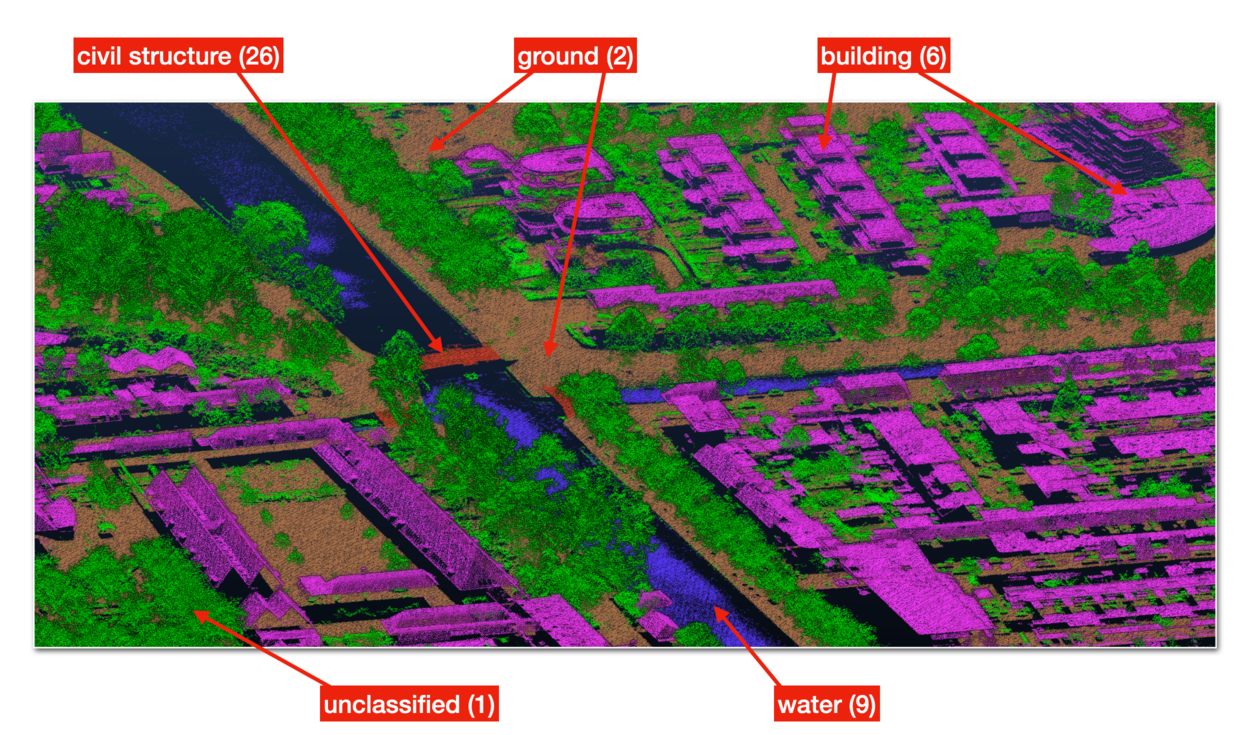
\includegraphics[width=\linewidth]{ahn4.png}
  \caption{Classification codes used in the AHN3+AHN4 datasets.}%
\label{fig:ahn3}
\end{figure}

Both AHN3 and AHN4 LAZ files use the ``Point Data Record Format 1'', which contains all fields from Format 0 (Table~\ref{tab:las-record}) with the addition of the GPS time of the measurement.
LAS v1.4 allows to store certain extra user-defined attributes, and in AHN4 the following 3 are also stored:
\begin{enumerate}
  \item \emph{Amplitude:} echo signal amplitude [dB] (min: 0; max: 10000) 
  \item \emph{Reflectance:} echo signal reflectance [dB] (min: 0; max: 10000)
  \item \emph{Deviation:} pulse shape deviation (min: 0; max: 65535)
\end{enumerate}

%


The national Dutch AHN lidar dataset 
\marginnote{\emph{Actueel Hoogtebestand Nederland} (AHN)}
\marginnote{\url{https://www.ahn.nl}}
is disseminated in the LAZ format (a compressed LAS, see below) and uses the LAS classification codes. 
Figure~\ref{fig:ahn3} shows all the codes that are used in both AHN3 and AHN4 (they are the same). 
Notice that apart from the pre-defined codes from Table~\ref{tab:las-classes}, it also uses the custom code $26$ for a `civil structure' (Dutch: \emph{kunstwerk}) class that includes special infrastructures such as bridges, statues, and viaducts. 

Notice that in AHN the points representing vegetation are not classified as such, and vegetation is never explicitly classified.
\marginnote{vegetation is classified as $1$/unclassified}
The is because the aim of the AHN project is mostly to model dikes and to protect us from floods, and vegetation is not very important for this use-case.
The class $1$ is thus used for vegetation, but other objects such as street furniture (\eg\ lampposts) or cars are also classified as $1$.

%

Certain tiles contain a new classification (\emph{high-voltage pylons and cables} == class 14), but not all of them. 
\marginnote{Class=14 for pylons+cables (for some tiles only)}
If 14 is not used, the pylons and cables are in class 26.

%


